\documentclass[10pt]{article}
\usepackage[utf8]{inputenc}
\usepackage[T1]{fontenc}
\usepackage{graphicx}
\usepackage[export]{adjustbox}
\graphicspath{ {./images/} }
\usepackage{amsmath}
\usepackage{amsfonts}
\usepackage{amssymb}
\usepackage[version=4]{mhchem}
\usepackage{stmaryrd}

\begin{document}
\section*{CT1 Exercises for Branching Instructions}
\section*{Content}
CT1 Exercises for Branching Instructions ..... 1\\
Exercise 1 - Unconditional Branches ..... 2\\
Exercise 2 - Conditional Branches ..... 3\\
Exercise 3 - Comparison Instructions ..... 4\\
Solutions ..... 5\\
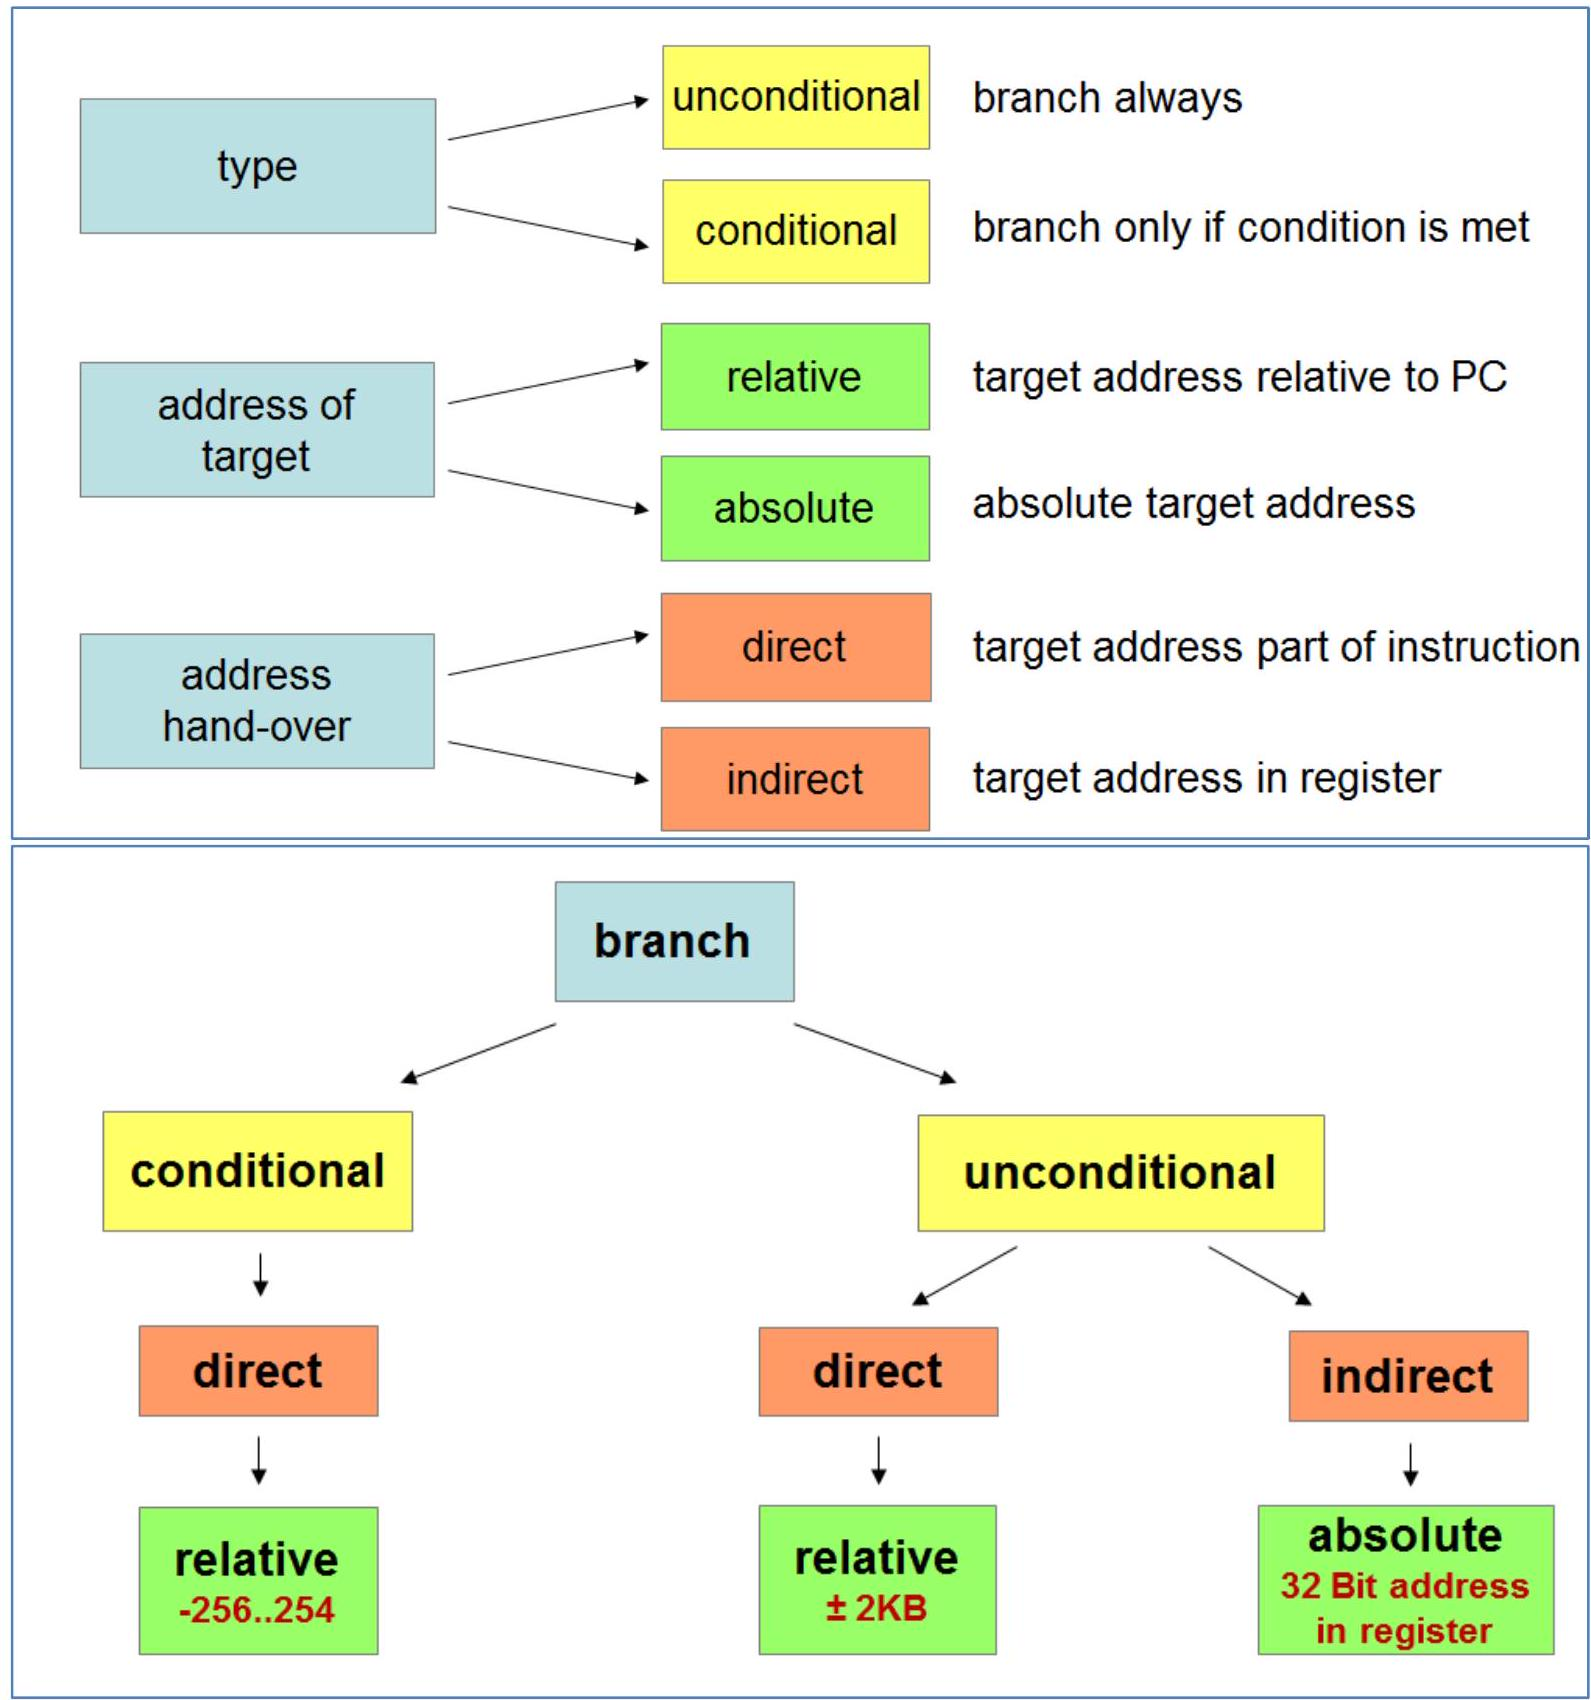
\includegraphics[max width=\textwidth, center]{2025_01_02_9902c2d2685de638ef73g-1}

\section*{Exercise 1 - Unconditional Branches}
The execution starts at line 10.

\begin{enumerate}
  \item List the sequence of branch instructions that end in an infinite loop.
\end{enumerate}

Do this by stating the branches in tabular form: from - to.\\
E.g. the first branch is $\underline{\mathbf{1 1 - 1 6}}$ (branch unconditionally from line 11 to line 16).\\
2) At which line does the execution sequence finally loop forever?

\begin{center}
\begin{tabular}{|l|lll|}
\hline
10 & Label1 & LDR & R0, =Label5 \\
11 & Label2 & BX & R0 \\
12 & Jumptable & DCD & Case0 \\
13 &  & DCD & Case1 \\
14 &  & DCD & Case2 \\
15 &  & DCD & Case3 \\
16 & Label5 & LDR & R0, =Label6 \\
17 &  & B & Label2 \\
18 & Label6 & LDR & R2, =Jumptable \\
19 &  & ADDS R2, R2, \#4 &  \\
20 & Label4 & LDR R2, [R2] &  \\
21 &  & BX & R2 \\
22 & Case0 & B & Case0 \\
23 & Case1 & LDR & R2, =Jumptable \\
24 &  & MOVS R1, \#3 &  \\
25 &  & LSLS R1, R1, \#2 &  \\
26 &  & ADDS R2, R2, R1 &  \\
27 &  & B & Label4 \\
28 & Case2 & B & Label1 \\
29 & Case3 & B & Case0 \\
\hline
\end{tabular}
\end{center}

Your solution (the number of cells below is no hint)\\
1)

\begin{center}
\begin{tabular}{|l|l|l|l|l|l|l|l|}
\hline
$11-16$ &  &  &  &  &  &  &  \\
\hline
\end{tabular}
\end{center}

2.

\section*{Exercise 2 - Conditional Branches}
The execution starts at line 10.

\begin{enumerate}
  \item List which branch instructions jump to the given label.
\end{enumerate}

Do this by stating the branches in tabular form: from - to.\\
2) What is the final value in $R 0$ as hexadecimal value?\\
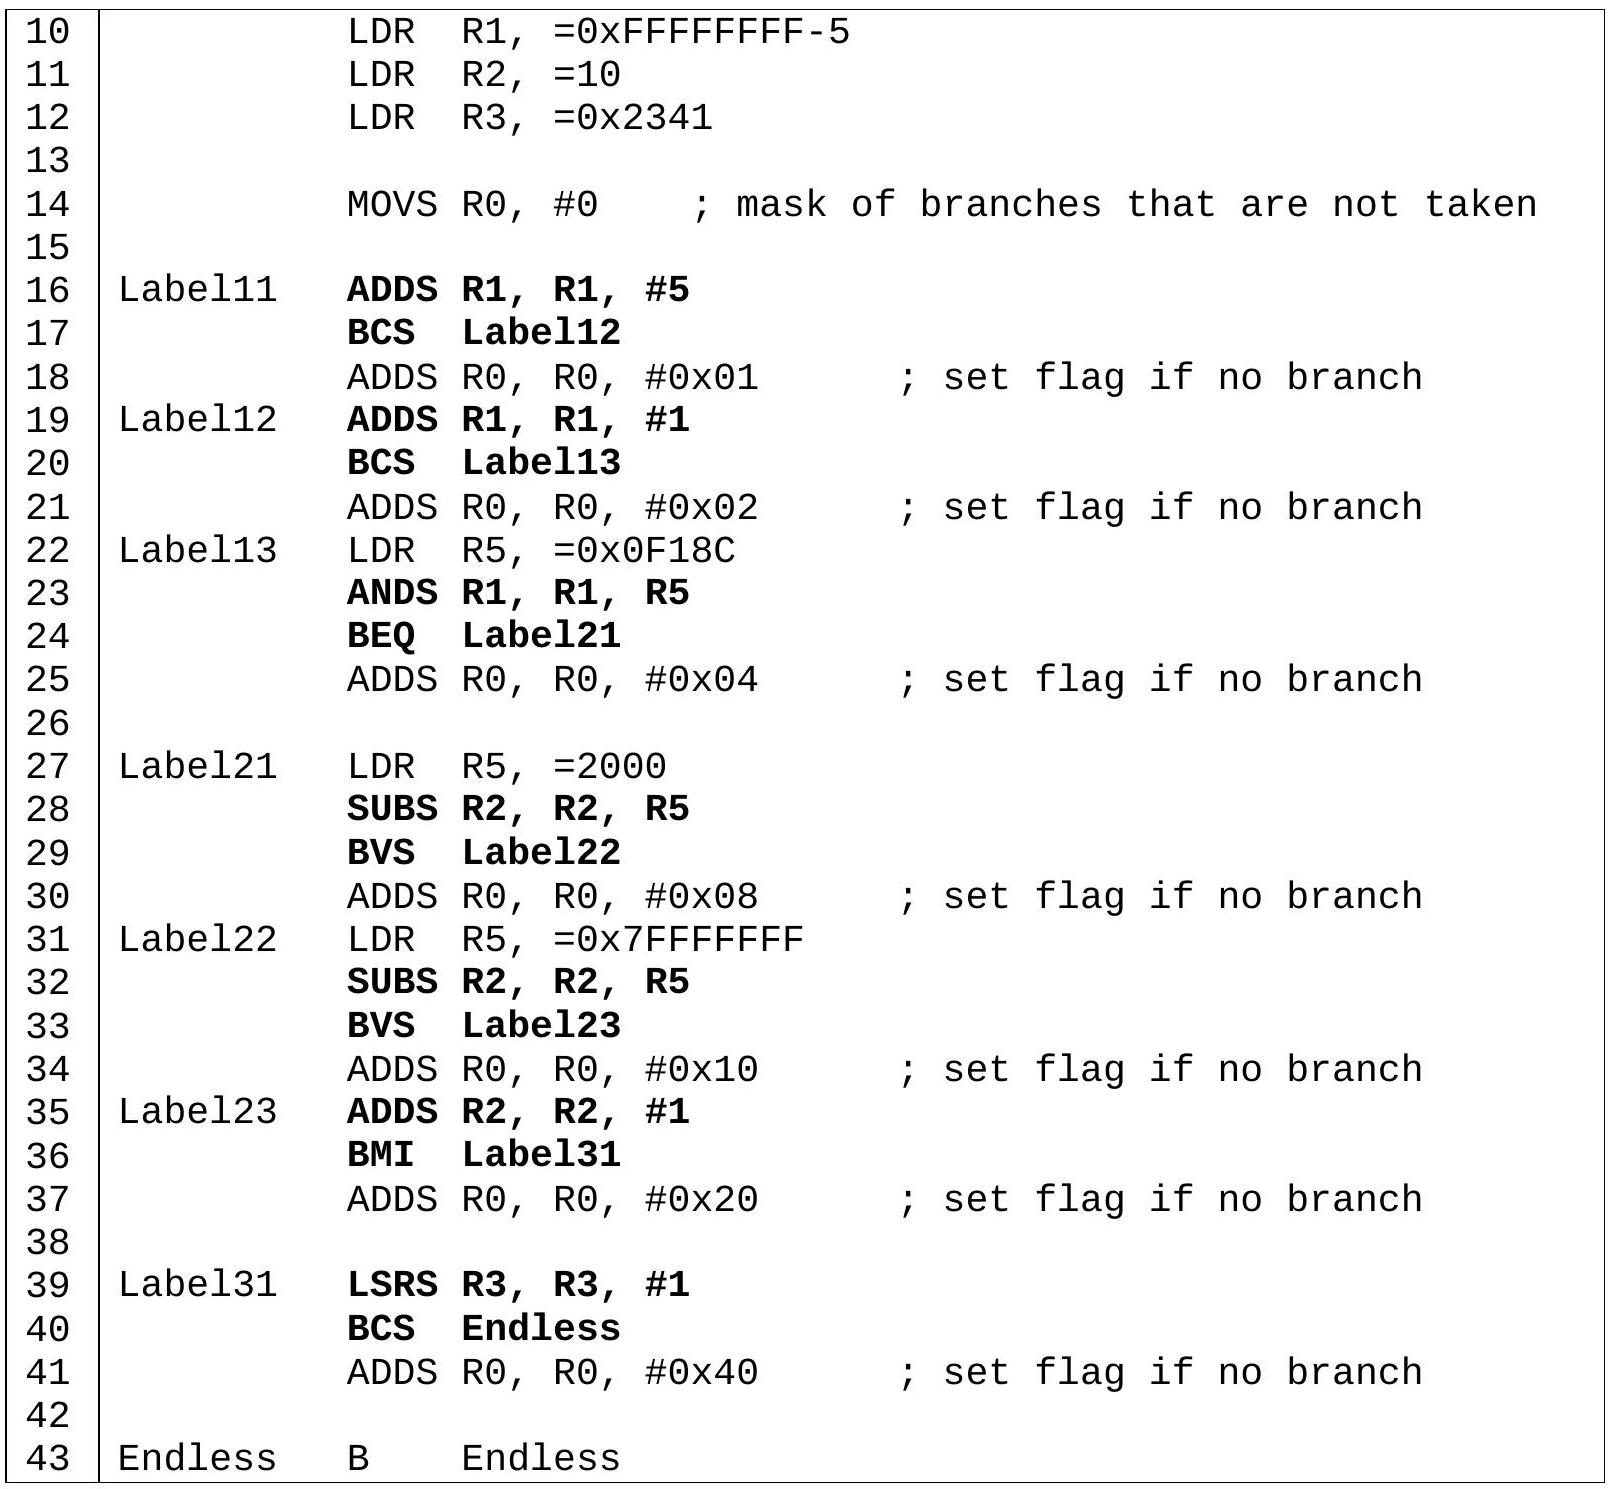
\includegraphics[max width=\textwidth, center]{2025_01_02_9902c2d2685de638ef73g-3}

Your solution (the number of cells below is no hint)

\begin{enumerate}
  \item $\square$
  \item $\quad R 0=0 x$. $\qquad$
\end{enumerate}

\section*{Exercise 3 - Comparison Instructions}
The execution starts at line 10.

\begin{enumerate}
  \item List which branch instructions jump to the given label.
\end{enumerate}

Do this by stating the branches in tabular form: from - to.\\
2) What is the final value in $R 0$ as hexadecimal value?\\
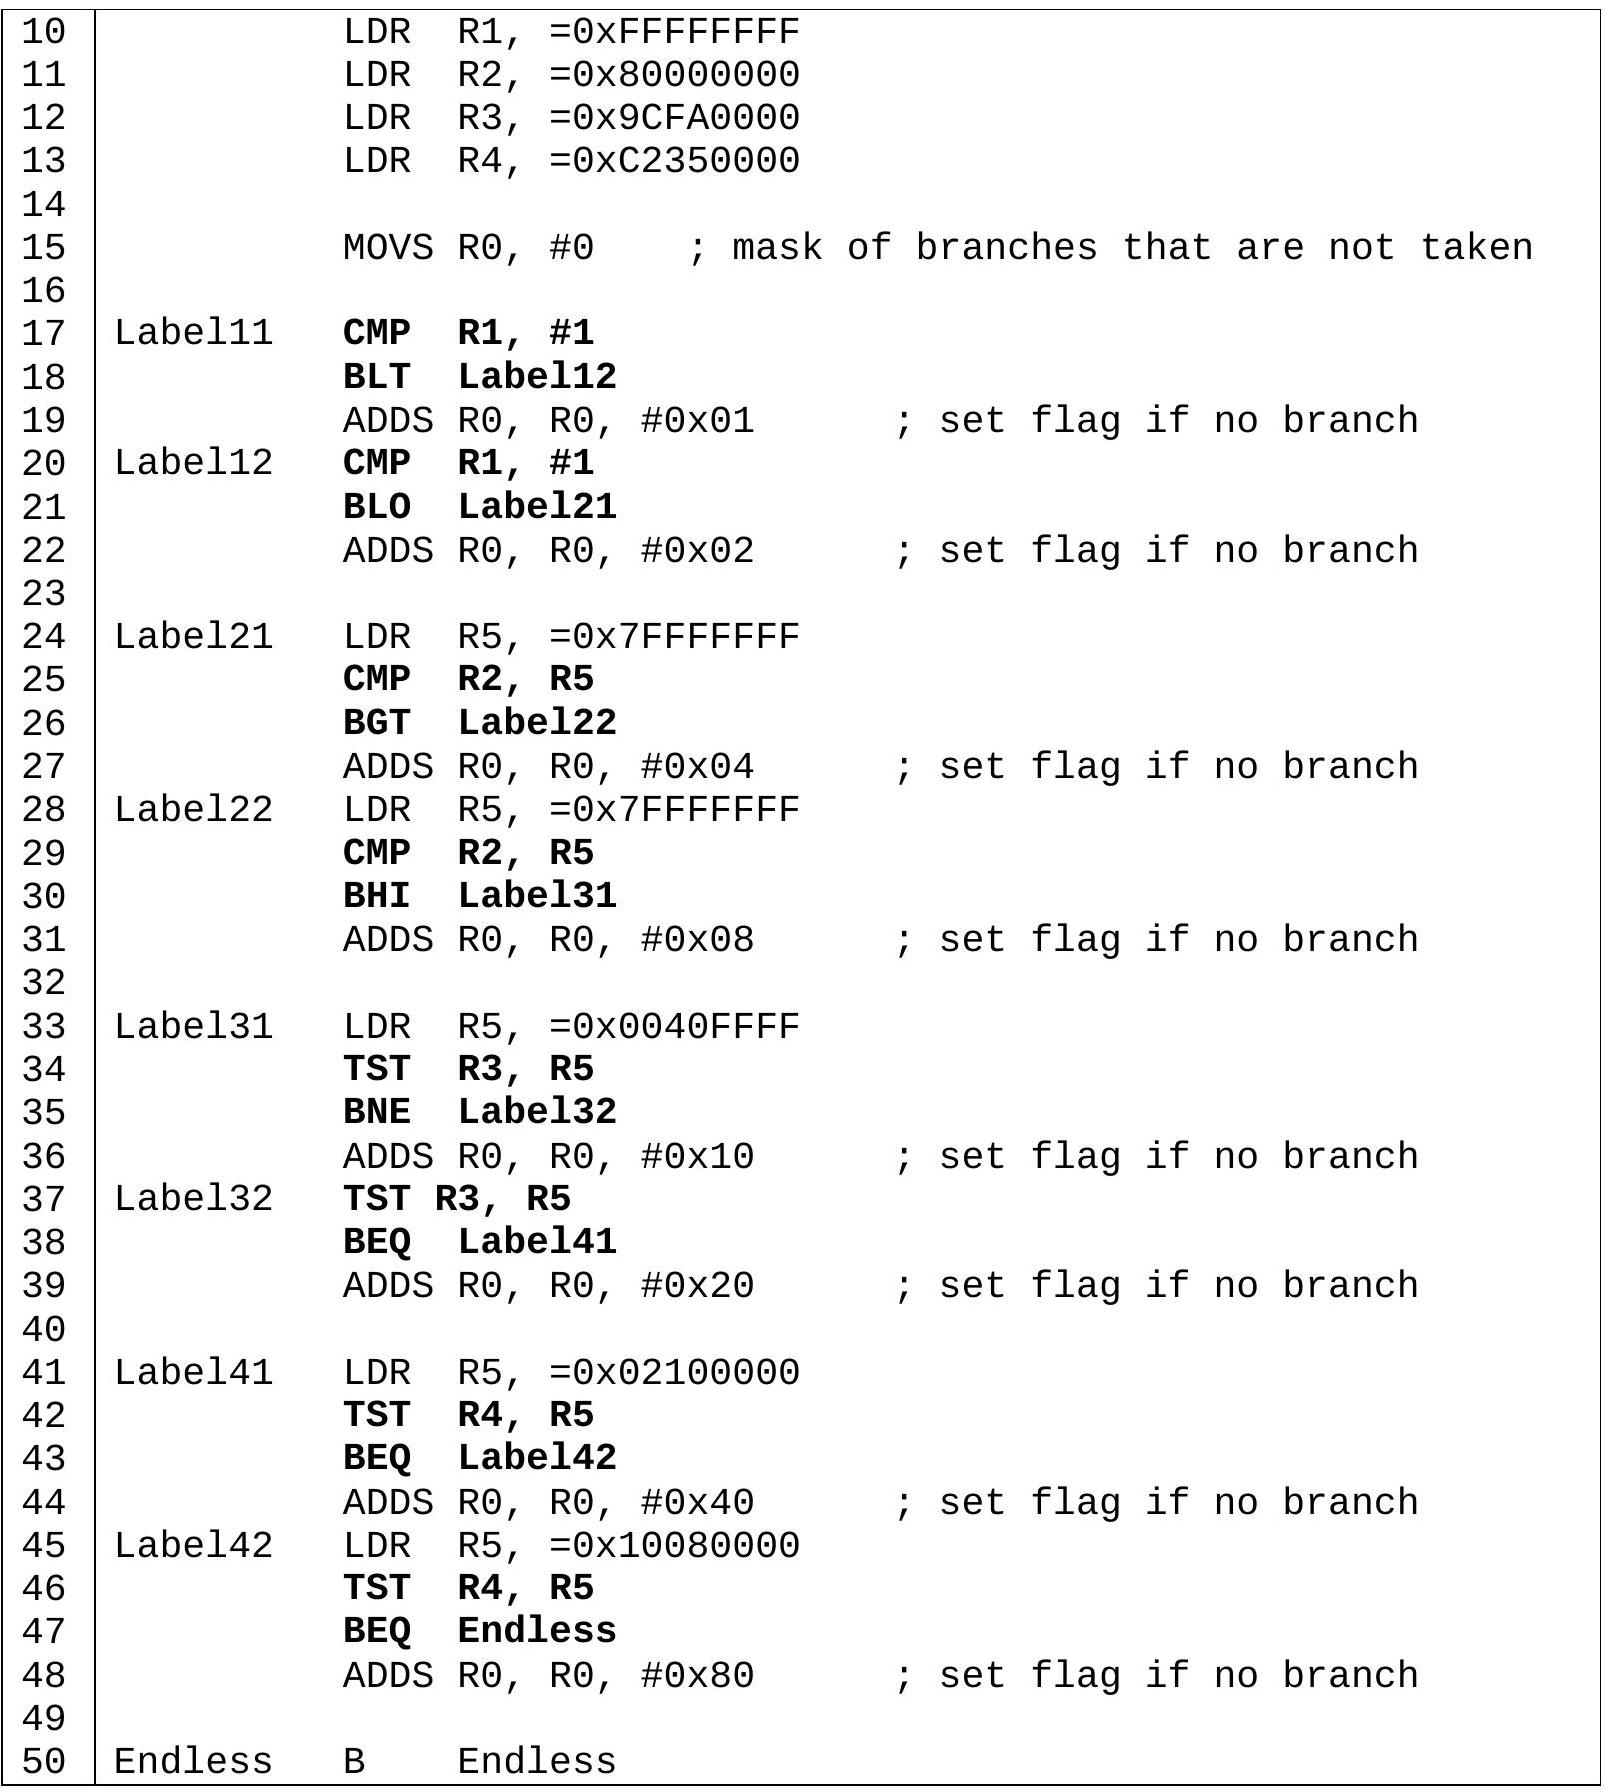
\includegraphics[max width=\textwidth, center]{2025_01_02_9902c2d2685de638ef73g-4}

Your solution (the number of cells below is no hint)

\begin{enumerate}
  \item $\square$
  \item $\quad R O=0 x$. $\qquad$
\end{enumerate}

\section*{Solutions}
\section*{Exercise 1:}
\begin{enumerate}
  \item $10-16,17-11,11-18,21-23,27-20,21-29,29-22,22-22 \ldots$
  \item Loops at line 22
\end{enumerate}

\section*{Exercise 2:}
\begin{enumerate}
  \item $20-22,24-27,33-35,40-43$
  \item $0 \times 29$ (binary 0010 '1001)
\end{enumerate}

\section*{Exercise 3:}
\begin{enumerate}
  \item $18-20,30-33,35-37,47-50$
  \item $0 \times 66$ (binary 0110 '0110)
\end{enumerate}

\end{document}